\section{Results}\label{sec:results}
	At a first stage, yeast and lactic bacteria monocultures were simulated to verify whether they work independantly of each other.
	At the second stage, the coculture was simulated to show.
	
	The mediums used contain \SI{50}{\litre} of water mixed with an inital glucose concentration of \SI{1000}{\milli\mole\per\litre}.
	\subsection{Yeast Monoculture}
		The yeast monocolture is well-behaved, until the very edges of metabolic activity, where the GEM is blocked.
		But its growth is almost exponential, as can be seen in Figure \ref{fig:yeast_0lac_pop}.
		The steep curve at the beginning marks the region where oxygen can be metabolised.
		The slight curvature of the following section can be explained by the self-inhibition of the organism,
		caused by the toxicity of ethanol, and by the sinking glucose concentration.
		Concentrations of the relevant metabolites that can be seen in Figure \ref{fig:yeast_0lac_met}
		
		At time $t\approx 25$ the GEM is blocked since the glucose uptake can not satisfy the ATP maintenance reactions anymore;
		the population starts to die.
		\begin{figure}[h]
			\centering
			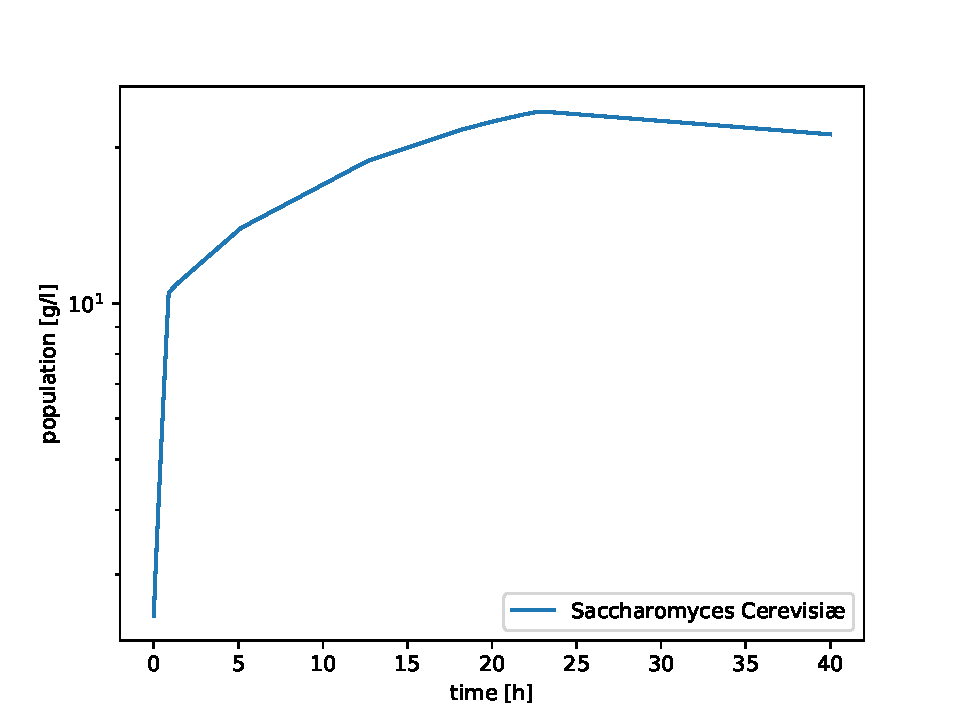
\includegraphics[width=\linewidth]{figures/results/yeast/0lac_populations.pdf}
			\caption{The yeast growth in the medium in a logarithmic scale}
			\label{fig:yeast_0lac_pop}
		\end{figure}
		\begin{figure}[h]
			\centering
			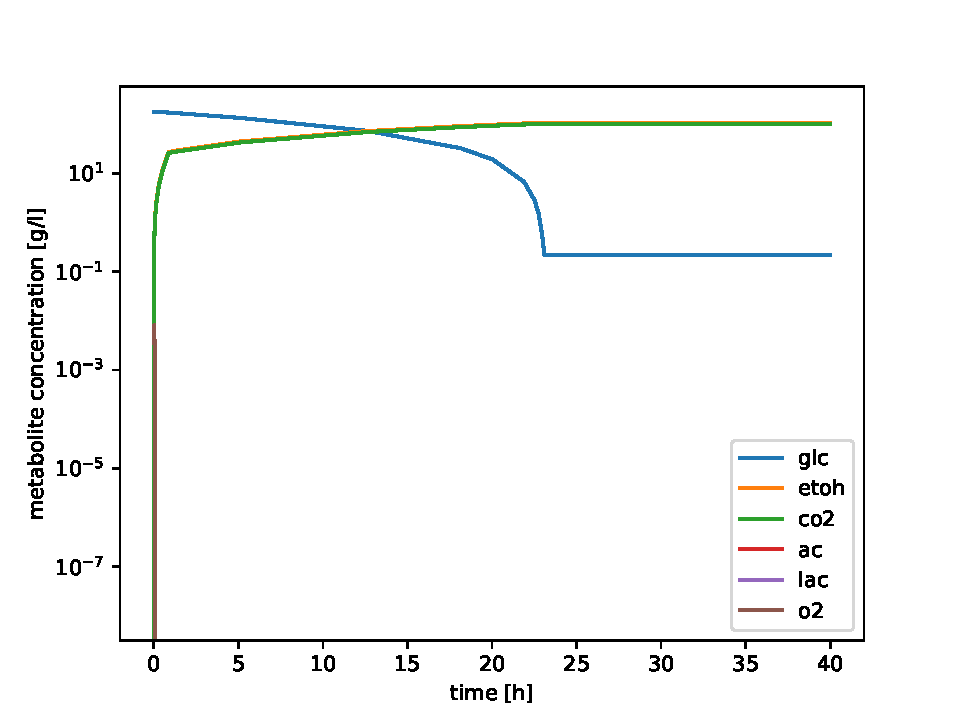
\includegraphics[width=\linewidth]{figures/results/yeast/0lac_metabolites.pdf}
			\caption{The concentrations of interesting metabolites in the simulated medium for yeast monocultures}
			\label{fig:yeast_0lac_met}
		\end{figure}
		
		In further simulations the concentration of lactate was increased, and the toxicity of the lactate was tuned to best fit the curves given in Figure \ref{fig:yeast_real}.
		This was achieved with a number of $I_{Y,\mathrm{glc,lac}}=\SI{30}{\milli\mole\per\litre}$. The Figure \ref{fig:yeast_simfig} shows the tuned curves.
		
		The fit is not perfect on multiple accounts: Firstly, the organism takes longer to metabolise the glucose, which can be traced back to a too high ethanol inhibition constant $i_{Y,\mathrm{glc,etoh}}$
		Secondly, there are sharp, seemingly non-smooth corners in the plot. These can be explained by wrong Michaelis-Menten constants $k_{Y,m}$
		
		Adapting these constants to $k_{Y,\mathrm{glc}}=\SI{15}{\milli\mole\per\litre}$ and the inhibition constant to $I_{Y,\mathrm{glc,etoh}}=\SI{350}{\gram\per\liter}$ yields a better fitting result
		shown in Figure \ref{fig:yeast_better_simfig}
		
		For the remainder of the simulations, the constants were reset to the original values.
		
		\begin{figure}[h]
			\centering
			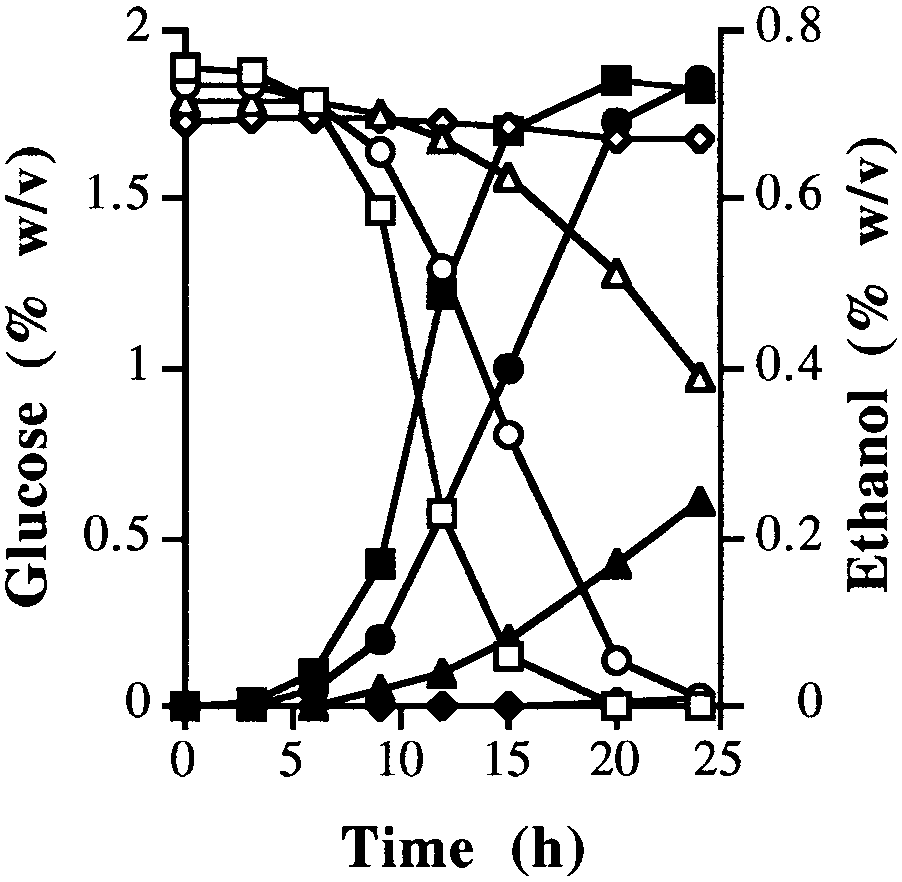
\includegraphics[width=0.6\linewidth]{figures/yeast_real.png}
			\caption{Glucose and ethanol concentrations measured in a real-life scenario with varying lactate concentrations \cite{Narendranath2001}. }
			\label{fig:yeast_real}
		\end{figure}
		
		\begin{figure}[h]
			\centering
			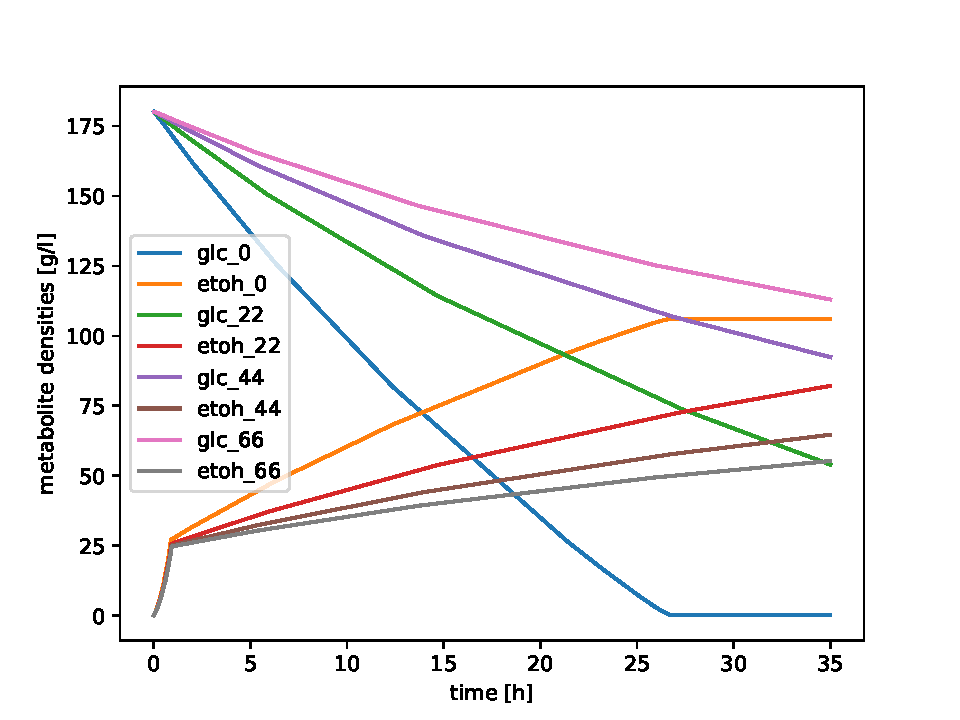
\includegraphics[width=\linewidth]{figures/results/yeast/similar_plot.pdf}
			\caption{The ethanol and glucose concentration at different concentrations of lactate}
			\label{fig:yeast_simfig}
		\end{figure}

		\begin{figure}[h]
			\centering
			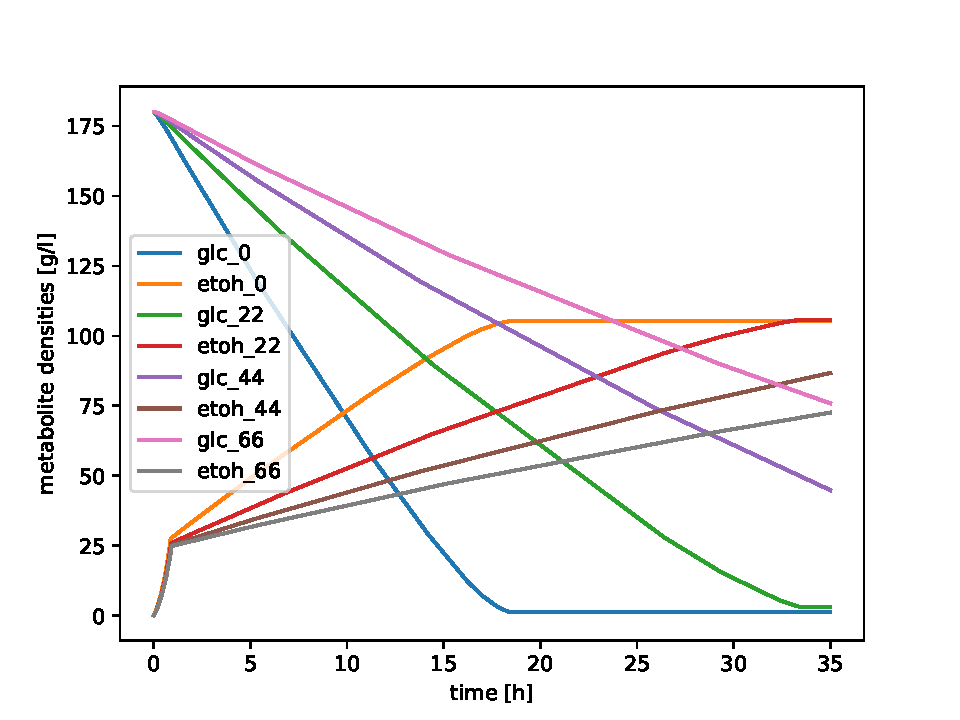
\includegraphics[width=\linewidth]{figures/results/better_yeast/similar_plot.pdf}
			\caption{The ethanol and glucose concentration at different concentrations of lactate with the improved constants}
			\label{fig:yeast_better_simfig}
		\end{figure}
		
	\subsection{Lactobacillus Plantarum}
		If we add Lactobacillus Plantarum to the same medium without the yeast, we get the population curves in Figure \ref{fig:lb_pop}.
		These, too, are what can be expected (i.e. exponential growth that gets dampened as the glucose runs out and ad the environment becomes more toxic).
		
		An interesting side-effect of the Lactobacilli is that they not only produce lactate and acetate, but also a rather large amount of ethanol.
		\begin{figure}[h]
			\centering
			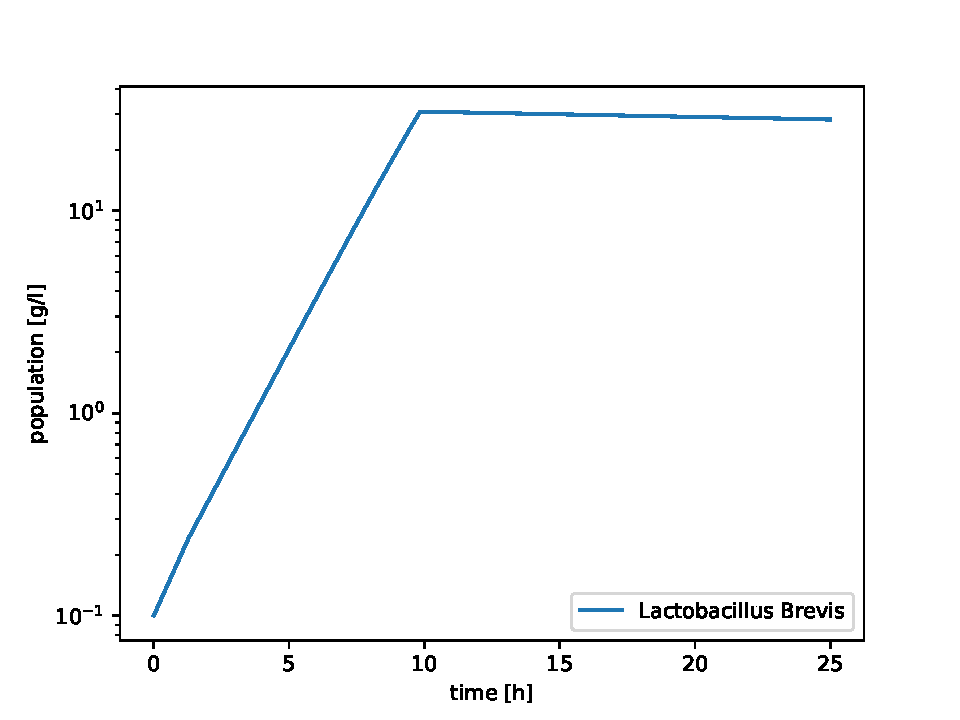
\includegraphics[width=\linewidth]{figures/results/lactobacillus/lactobacillus_populations.pdf}
			\caption{The growth of Lactobacillus Plantarum in the medium in a logarithmic scale}
			\label{fig:lb_pop}
		\end{figure}
		
		\begin{figure}[h]
			\centering
			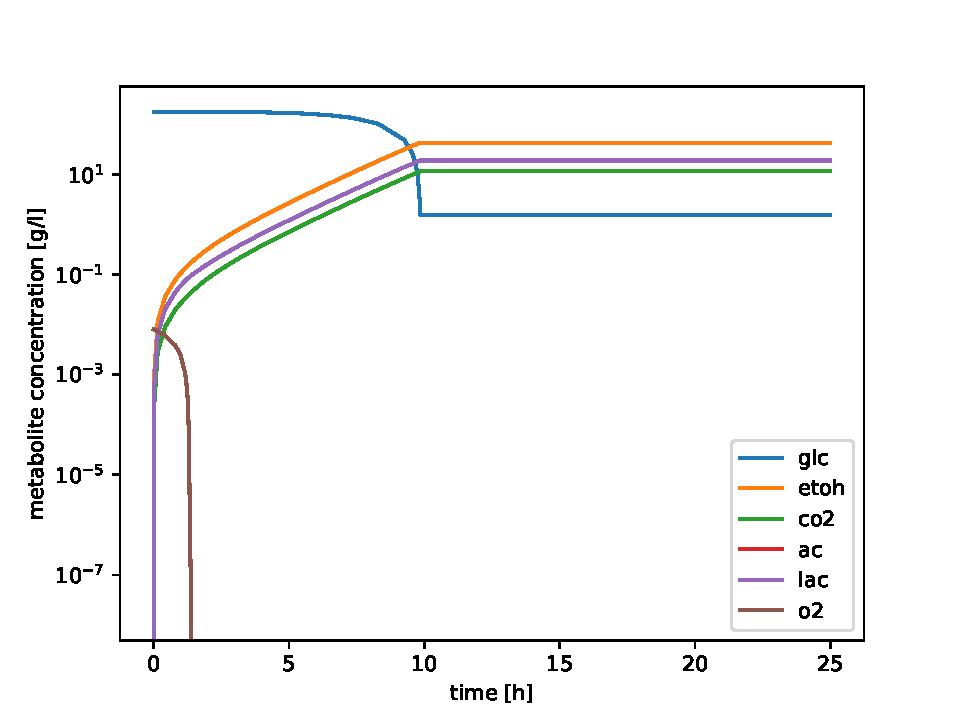
\includegraphics[width=\linewidth]{figures/results/lactobacillus/lactobacillus_metabolites.pdf}
			\caption{The concentrations of interesting metabolites in the simulated medium for Lactobacillus Plantarum monocultures}
			\label{fig:lb_met}
		\end{figure}
	
	\subsection{Cocultures}
		The simulation of the cocultures shows many effects known by experiment.
		The yeast shows much higher activity relative to the lactic bacteria when the medium contains oxygen, as can be seen in both Figure \ref{fig:cocult_0.1_met} and \ref{fig:cocult_1_met}.
		This is congruent with the common brewing practice of aerating the wort before actually fermenting it \cite[P. 168]{daniels1996designing}.
		More oxygen gives the yeast an additional head start in population.
		
		Additionally, whether the Lactobacilli overtake the yeast is dependant on the initial concentration of Lactobacillus Plantarum.
		This can be seen in Figure \ref{fig:cocult_pops}.
		
		\begin{figure}[h]
			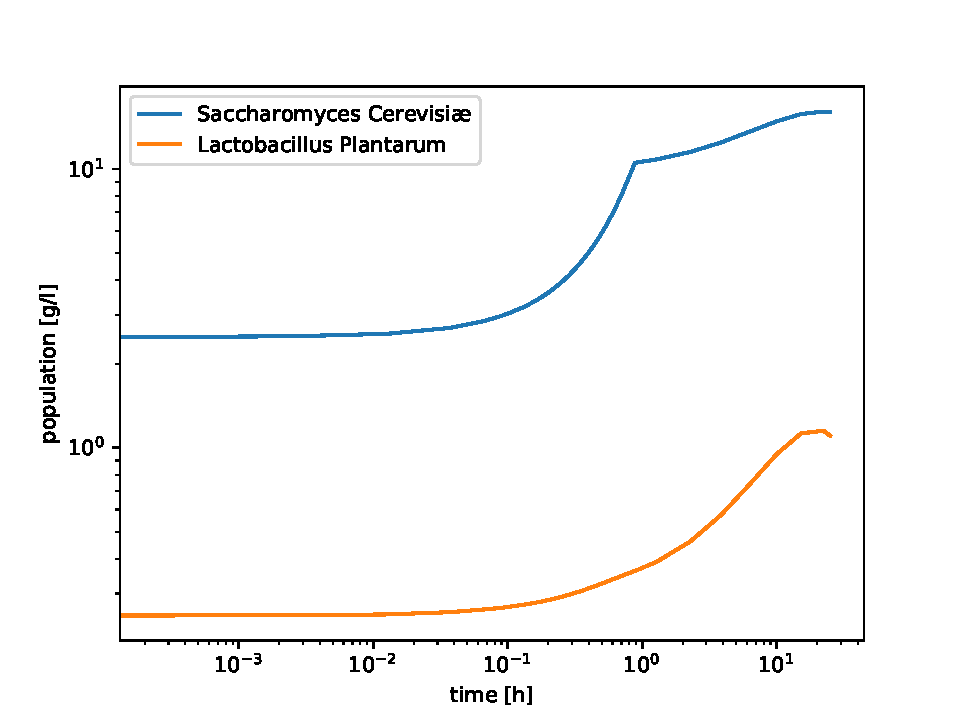
\includegraphics[width=\linewidth]{figures/results/cocultures/0_1_populations.pdf}
			\caption{The population of the two organisms with \SI{0.05}{\gram\per\litre} initial lactobacillus population}
			\label{fig:cocult_0.1_pop}
		\end{figure}
		
		\begin{figure}[h]
			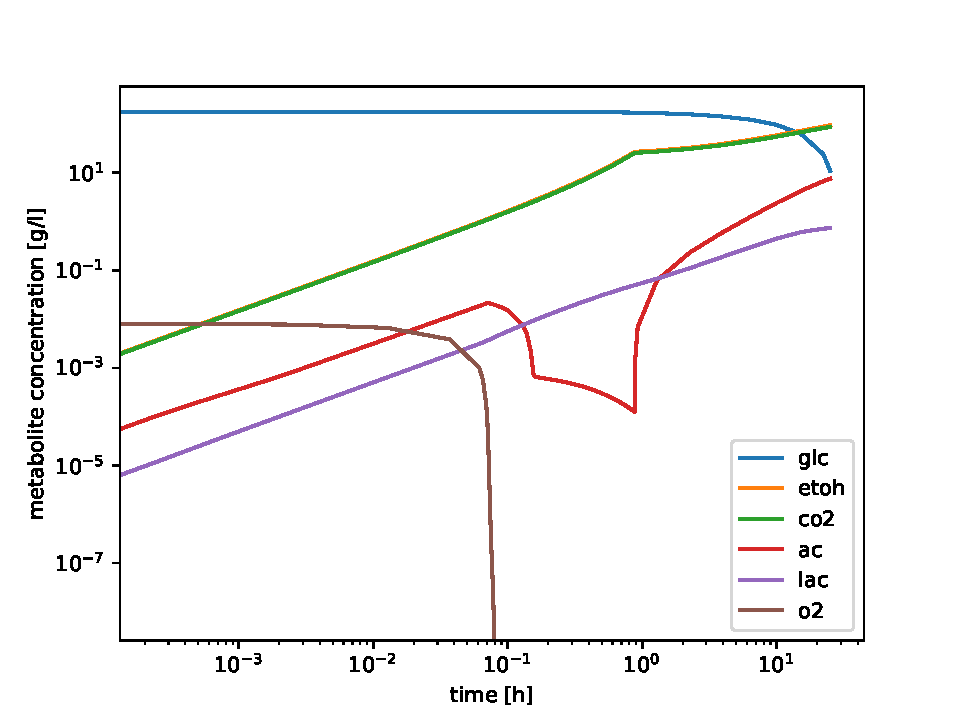
\includegraphics[width=\linewidth]{figures/results/cocultures/0_1_metabolites.pdf}
			\caption{The metabolites in the medium with \SI{0.05}{\gram\per\litre} initial lactobacillus population}
			\label{fig:cocult_0.1_met}
		\end{figure}
		
		\begin{figure}[h]
			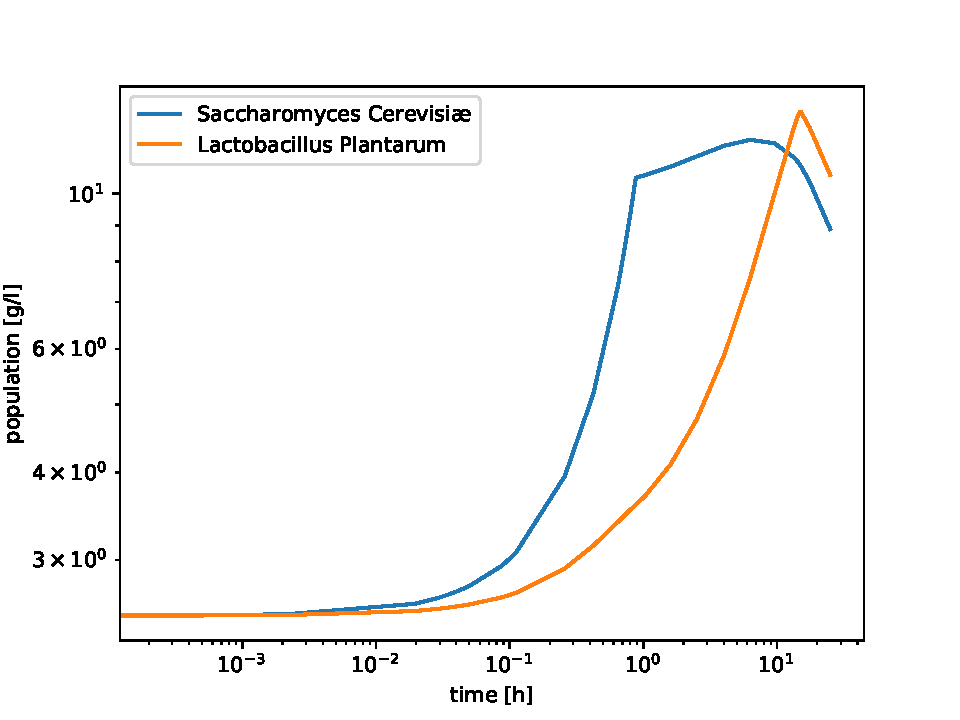
\includegraphics[width=\linewidth]{figures/results/cocultures/1_populations.pdf}
			\caption{The population of the two organisms with \SI{0.5}{\gram\per\litre} initial lactobacillus population}
			\label{fig:cocult_1_pop}
		\end{figure}
		
		\begin{figure}[h]
			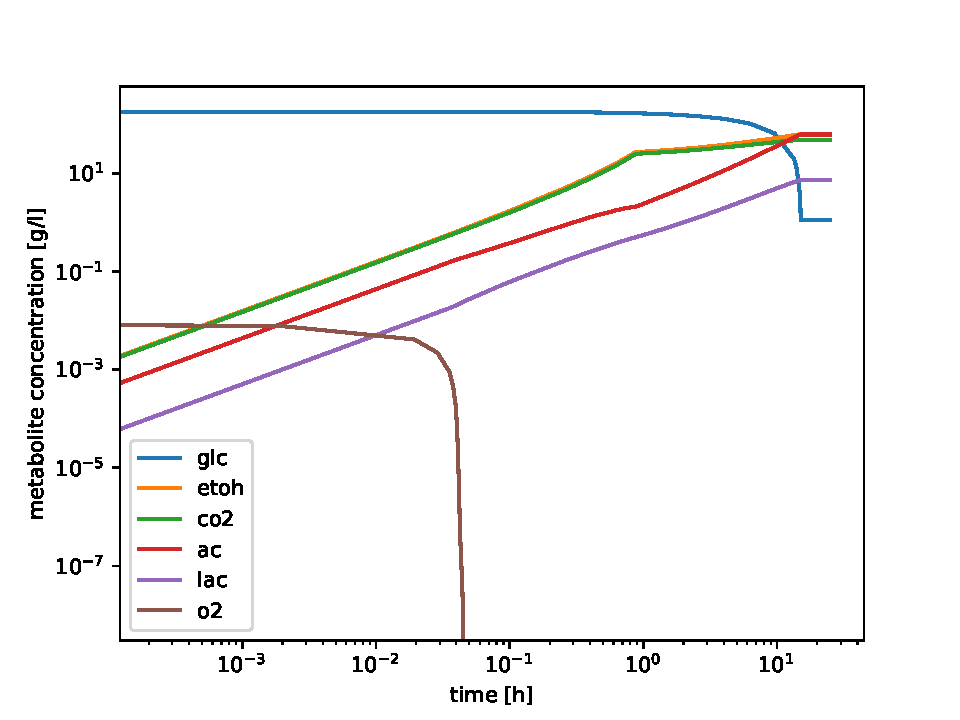
\includegraphics[width=\linewidth]{figures/results/cocultures/1_metabolites.pdf}
			\caption{The metabolites in the medium with \SI{0.5}{\gram\per\litre} initial lactobacillus population}
			\label{fig:cocult_1_met}
		\end{figure}
		
		\begin{figure}[h]
			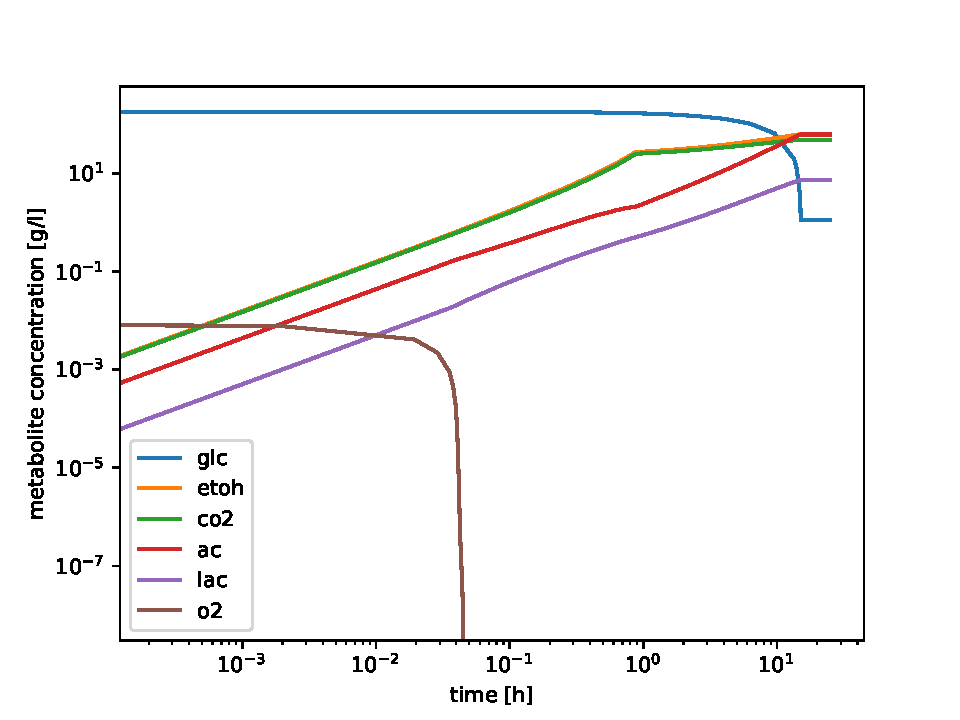
\includegraphics[width=\linewidth]{figures/results/cocultures/1_metabolites.pdf}
			\caption{The populations over multiple initial Lactobacillus concentrations (0.05, 0.5, 5, 50)}
			\label{fig:cocult_pops}
		\end{figure}
